\chapter{Neural models for the perceptual organization of 3D surfaces}
\label{sec:surfaces}
\chaptermark{3D Surface Representation}

\section{Introduction}

Since we live in a complex 3D world, competent interaction with the surrounding 3D scene structure is indispensable to us and our machines. Access to information about surfaces present in the scene allows us to perform a wide variety of tasks, ranging from motor planning (\eg reaching for a cup a certain distance away on the table) to spatial navigation (\eg following directions in a new city environment).

In studying perceptual organization, researchers have traditionally relied on simple 2D stimuli such as oriented bars~\citep{Palmer_02}. Results from these studies provide support for the importance of well-known Gestalt principles~\citep{Koffka35, Wertheimer23}, for instance that visual elements are grouped together in a way that begins to give meaning to the visual scene (\eg figure \vs background). However, it is unclear how well the results from these relatively simple experiments generalize to the 3D objects and scenes regularly encountered in natural settings. Because we act in a 3D world, perceptual organization must also help to arrange 3D information in a way that can guide our actions. 

\begin{figure}[t]
\centering
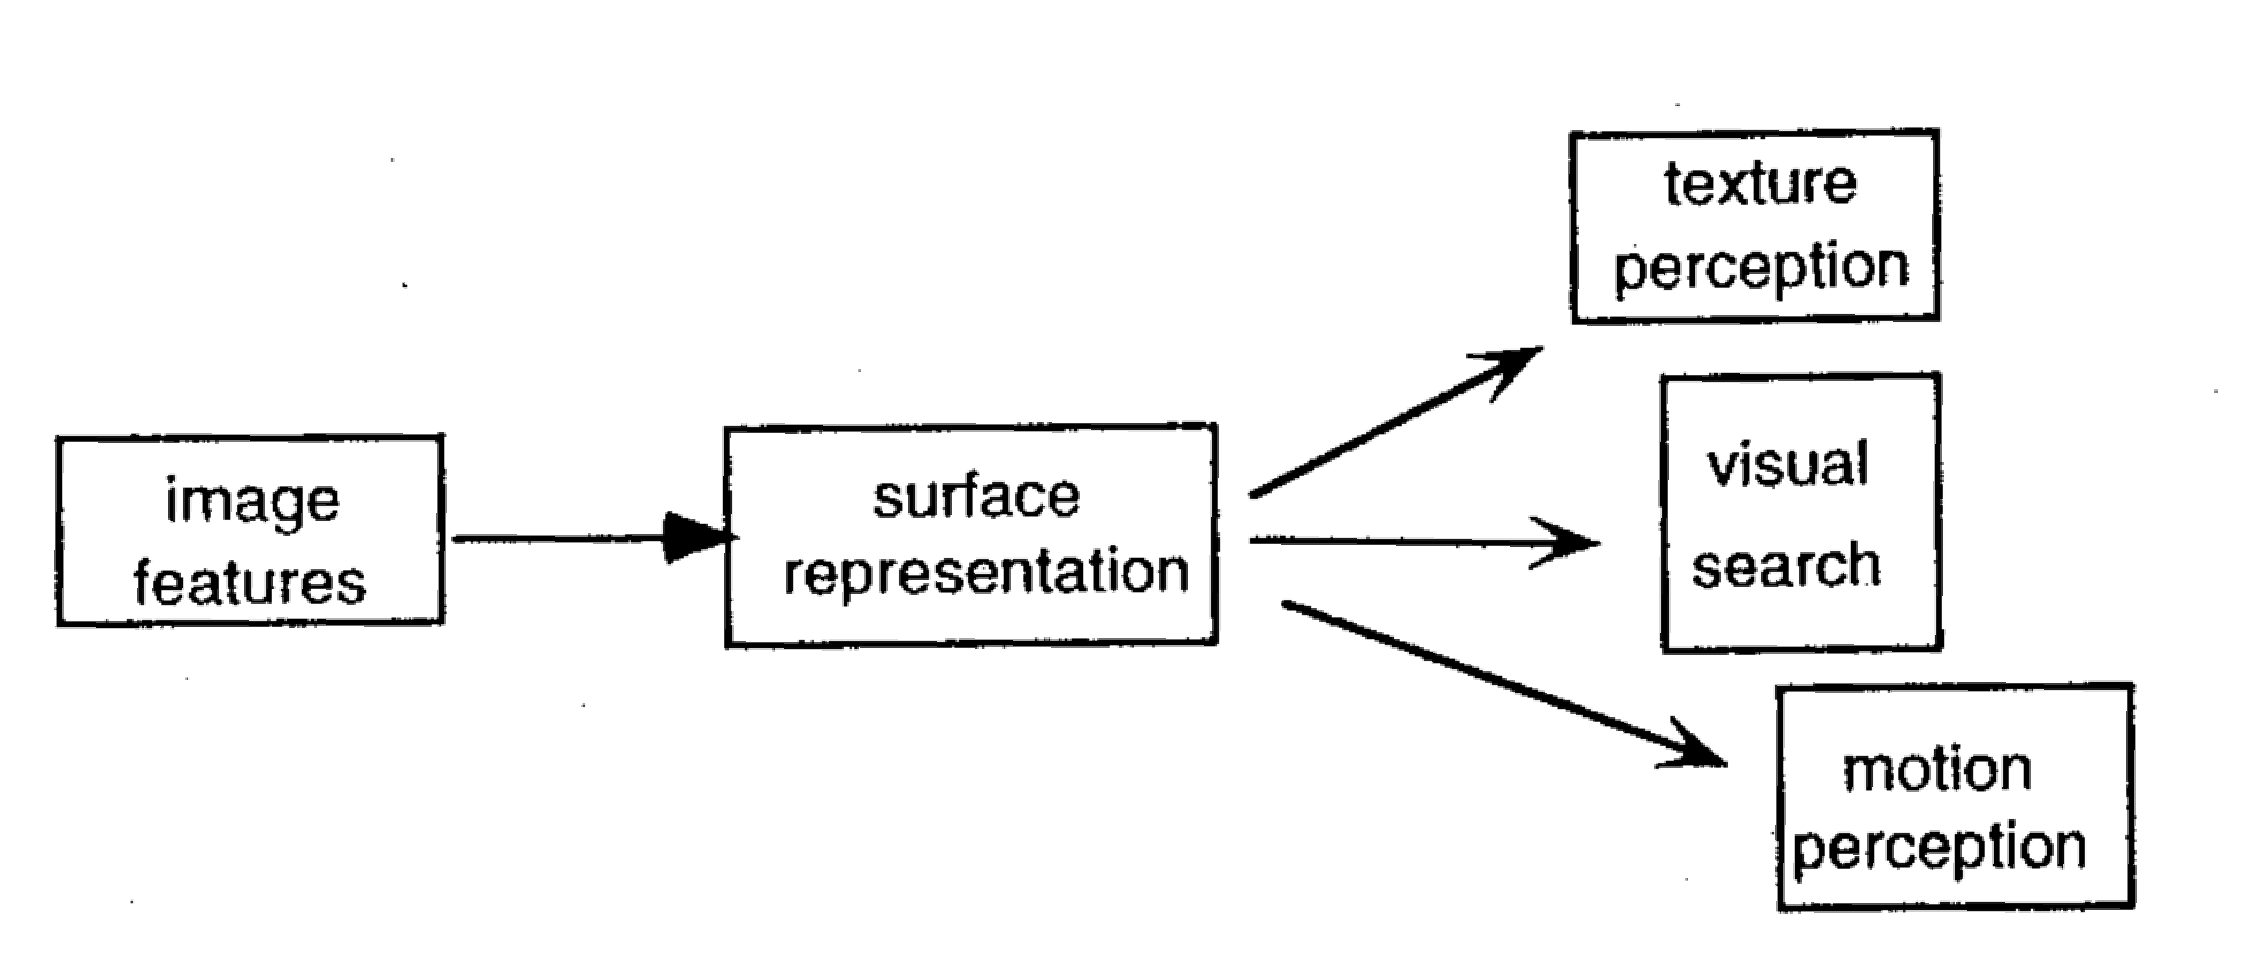
\includegraphics[width=0.75\textwidth]{3D-Surface/figs/nakayama_surface}
\makeatletter
\let\@currsize\normalsize
\caption[Surface representation precedes perceptual visual function]{The proposed view in which surface representation precedes perceptual functions such as texture perception, visual search, and motion perception. Reproduced from~\citet{Nakayama_etal95}.}
\label{NakayamaSurface}
\end{figure}

Perceptual organization also provides a structure for selectively attending to groups of objects~\citep{Treisman_Gelade80}. Supported by extensive psychophysical data,~\citet{Nakayama_etal95} proposed that surface representations play a key role in intermediate-level vision, 
%
providing a critical link
between lower-level and higher-level visual functions.
In the proposed view, image features give rise to surface representations that can be used for a variety of tasks, including texture perception, visual search, and motion perception (Figure~\ref{NakayamaSurface}).
% include Nakayama figure here
%
For example, subjects can perform efficient search for a conjunction target by selectively attending to the surface that the target is on in 3D space~\citep{Nakayama_Silverman86}. Attention has also been shown to spread automatically across surfaces in a separate cueing experiment~\citep{He_Nakayama95}. These abilities indicate powerful mechanisms for grouping objects into surfaces in 3D space, and suggest that structuring the world in terms of surfaces might be an ecologically important function. These results also have implications for the internal representation of surfaces, because they imply that the visual scene is processed in a way that preserves its 3D
structure. This representation must also be able to bring together
information from different sensory modalities (\eg vision, audition,
\etc), in order to form a common representation of the 3D environment
that is useful for an agent's behavioral goals~\citep{Lewicki_etal14}.

In addition to being studied by human psychophysical approaches, perceptual organization has been the subject of many studies in the visual system of non-human primates. Many neurons in early visual cortex encode the side to which an object border belongs, a phenomenon known as border ownership~\citep{Zhou_etal00}. Selectivity for the side of ownership involves integrating global context information about the object. Several models have been proposed~\citep{Zhaoping05, Craft_etal07} to describe how a neuron's border ownership selectivity can be modulated by visual input far away from its classical receptive field with the observed high specificity of object details. One view is that this contextual input is provided by feedback connections from ``grouping cells''~\citep{Craft_etal07} which bias the activity of border ownership cells and thus generate their context-dependent responses.~\citet{Mihalas_etal11b} have also shown that
grouping cells can direct and sharpen a broad attentional spotlight to the lower-level features of a specific object. In this chapter, we extend this grouping framework to 3D space to show how oriented 3D elements can be grouped into planar surfaces.

Currently, we know very little about how surfaces are represented in the brain, and how this representation is computed. Our model sheds light on a possible neural representation of 3D surfaces and relates this model to previous psychophysical results. Furthermore, we propose that the brain may use basis functions to flexibly and efficiently represent different surfaces using the same population of neurons.

\begin{figure}[t]
\centering
\includegraphics[width=0.75\textwidth]{3D-Surface/figs/groupingcircuit}
\makeatletter
\let\@currsize\normalsize
\caption[3D surface grouping model network]{Network structure, adapted from~\citet{Marshall_etal96}.}
\label{NetworkStructure}
\end{figure}

\section{Methods}

\subsection{Model of surface grouping}

An overview of the network structure of our model is shown in
Figure~\ref{NetworkStructure}. We extend a neural model of visual
stereomatching~\citep{Marshall_etal96} that is conceptually similar to
grouping models previously proposed for 2D stimuli~\citep{Craft_etal07, Mihalas_etal11b, Russell_etal14}. The model contains three layers of neurons. The first layer consists of monocular cells, which respond to visual features (e.g. spots, edges, {\em etc.}) presented to either the left or right eye. The input to the model consists of pairs of stereo images, as would be seen by the left and right eyes. In our model, we set the image input to a value of unity wherever a stimulus is present and zero elsewhere.

The second layer consists of binocular cells, which receive excitatory
input from monocular cells. These cells are tuned to a certain disparity based on a fixed spatial weighting between the left and right monocular cells, analogous to the disparity-selective binocular neurons in visual cortex of monkeys~\citep{Poggio_Fischer77, Poggio_Poggio84} and cats~\citep{Bishop_Pettigrew86, Ohzawa_etal90}. Lateral inhibition between cells representing different disparities along the same left- or right-eye line of sight reduces potential false matches~\citep{Marr_Poggio76}.

The third and final layer consists of planar grouping cells which receive excitatory input from populations of disparity-selective
cells. Receptive fields of the planar grouping cells are relatively broad and non-specific, resembling surface patches with a certain range of depth and orientation selectivity in 3D space. These cells may correspond to neurons found in parietal cortex, which have been shown to be selective for the tilt and slant of planar surfaces~\citep{Rosenberg_etal13}. In our model, we used a total of 15~planar grouping cells (\ie five frontoparallel planes, five back slant planes, and five front slant planes), which was sufficient to ``tile'' the whole 3D visual scene. Planar grouping cells compete with each other through lateral inhibition, which helps to select the best possible interpretation of surfaces within the scene. Additionally, planar grouping cells send reciprocal feedback connections to the disparity-selective cells that define their surface, akin to the relationship between grouping cells and border ownership cells in models of 2D scenes~\citep{Craft_etal07,Mihalas_etal11b}. To avoid
uncontrolled feedback excitation, feedback is multiplicative and only amplifies existing feedforward excitation. Selective attention is modeled as an additive input to those planar grouping neurons representing attended objects. This attentional modulation input is set to a value of 0.25 of the sensory input. A more detailed description of the model equations and parameters can be found in~.
% cite Appendix?

All model neurons are simulated as single compartment units with an
activity that is modeled as a continuous variable (rate coding). These
units are zero-threshold, linear neurons which receive excitatory and
inhibitory current inputs. The activity of the units is determined by
a set of coupled, first-order nonlinear ordinary differential equations, which can be solved in MATLAB (MathWorks) using standard numerical integration methods (Euler, Runge-Kutta, \etc) 

\begin{figure}[t]
\centering
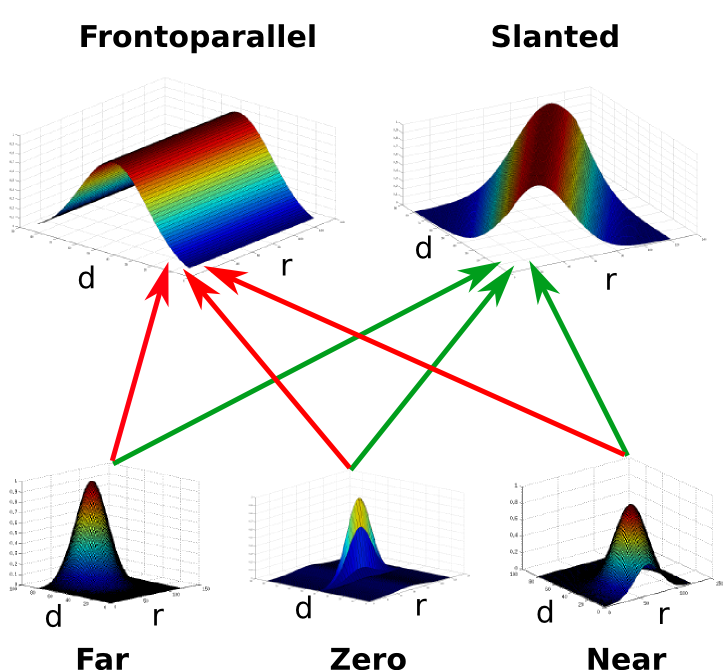
\includegraphics[width=0.75\textwidth]{3D-Surface/figs/basisfunc_new.png}
\makeatletter
\let\@currsize\normalsize
\caption[Basis functions can flexibly represent different surfaces using learned weights]{The same set of basis functions (\eg far, zero, and near-tuned units with disparity and retinotopic tuning) can be used to generate different surfaces. Learned weights can be used to represent a fronto-parallel surface (red arrows) or a slanted surface (green arrows).}
\label{Basis functions}
\end{figure}

\subsection{Disparity-selective cells as basis function units}
\label{sec:basis_func}

Orientation selective cells in V2 have gain field-like properties, with their responses to stimulus orientation depending nonlinearly on disparity~\citep{vonderHeydt_etal00a}.
\citet{Pouget_Sejnowski97b} showed that neurons in parietal cortex with gain fields can be used as basis functions of their sensory inputs for mapping different eye-hand coordinate transformations. Using identical mathematics, we propose that visual disparity (or depth) can play the same role as eye position, generating representations of planes of arbitrary orientations in 3D space. If a surface, $S$, is a nonlinear function of binocular disparity, $\vec{d}$, and retinotopic position, $\vec{r}$, it can be generated by a linear combination of basis functions spanning these two dimensions,

\begin{equation}
\mathcal{S} = \sum_{i}c_{i}B_{i}(\vec{d}, \vec{r})
\end{equation}

\noindent where $c_{i}$ are cofficients that can be learned depending on the surface, $S$, and $B_{i}$ are a set of basis function units with biologically-plausible receptive fields.

Figure~\ref{Basis functions}
%
%use figure showing basis functions
%
shows how the space of retinal position and depth is spanned by disparity-selective cells, which forms a set of basis functions. One axis is along binocular disparity ($\vec{d}$), the other is along retinal coordinates ($\vec{r}$); the latter are obviously two dimensional but only one dimension is shown. Three examples of disparity-selective cells are shown in the bottom row of the figure. From left to right, shown are receptive fields of three foveal cells selective for far disparity, central disparity, and near disparity, respectively. Obviously, these are examples only and a much larger number of cells is needed to span the space in detail. For our results, we used a total of 289 basis function units, $B_{i}$ , whose receptive fields were computed by multiplying Gaussian retinal receptive fields with disparity tuning curves. The peaks of the Gaussians were spread uniformly between $-4^{\circ}$ and $4^{\circ}$, in increments of $0.5^{\circ}$. The standard deviation of the Gaussian was fixed at $0.6^{\circ}$. The peaks of the disparity tuning curves were based on the minimal number of neurons required to reproduce psychophysical disparity discrimination curves, which was found to be 17~\citep{Lehky_Sejnowski90}. The exact formulation for the near, tuned, and far disparity tuning curves can be found in Table 1 of~\citet{Lehky_Sejnowski90}.
%~\citep[][used 121 basis functions]{Pouget_Sejnowski97b}.

Arrows in the figure indicate weighted connections that combine activity of basis function sets into new receptive fields of which two examples are shown at the top. The RF on the left is in the fronto-parallel plane at zero disparity. Planes with non-zero disparities (not shown) are parallel to it but displaced to the left or right in the figure. Top right is a RF that represents a surface slanted in space. In our model, neurons with receptive fields as in Figure~\ref{Basis functions} group features on surfaces in 3D space, in complete analogy to the grouping mechanisms in 2D employed in previous work~\citep{Craft_etal07,Mihalas_etal11b}. The weights of these connections, $c_{i}$, can be learned by traditional supervised learning techniques, \eg the delta rule~\citep{Widrow_Hoff60}. The training set was composed of 49 pairs of retinal position and disparity, selected from within the range $-3^\circ{}$ and $3^\circ{}$ for both values. Weights were adjusted until the mean squared error (MSE) of our approximation to the actual values was less than 0.001.

\begin{figure}[t!] % consider splitting this horizontally to save space
\centering
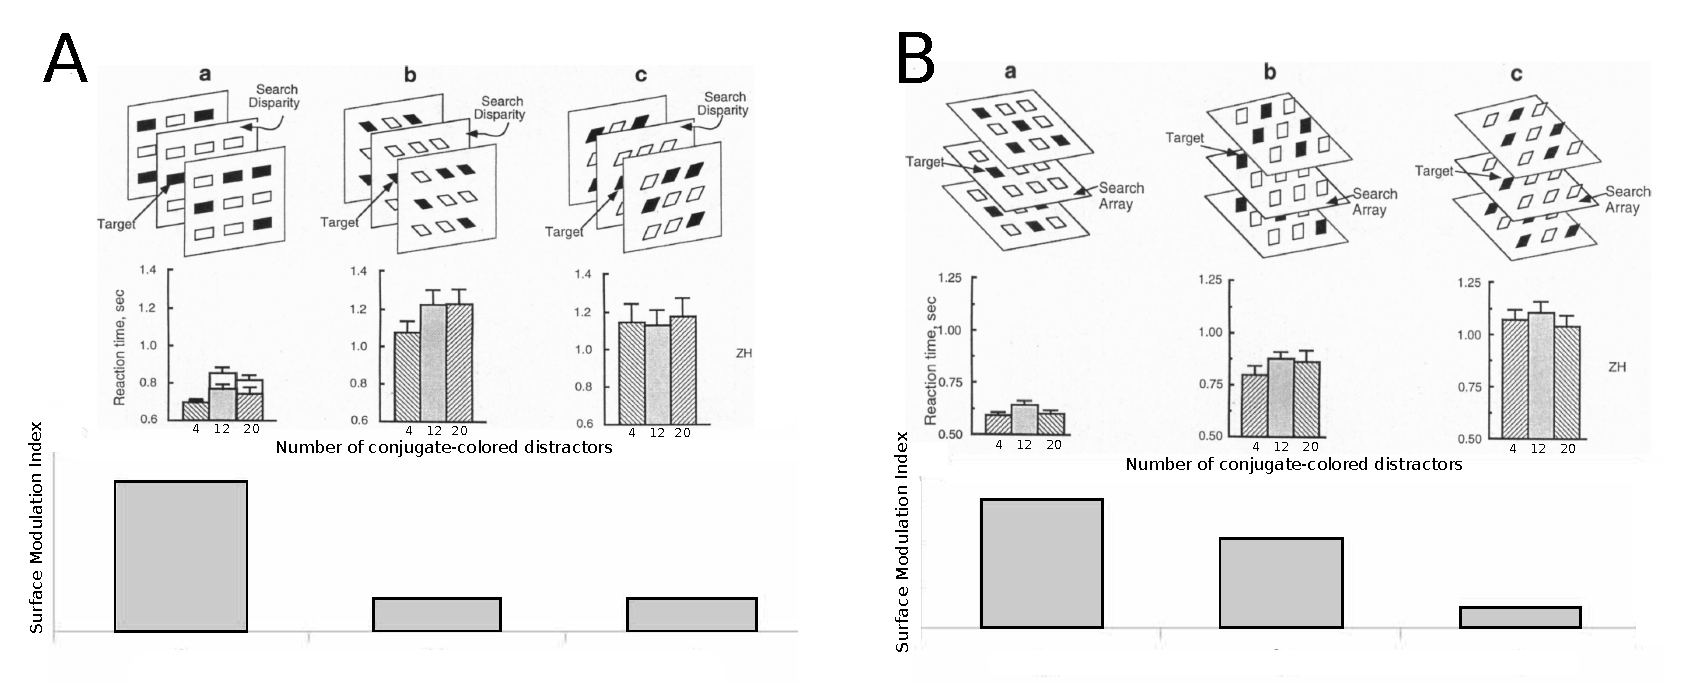
\includegraphics[width=\textwidth]{3D-Surface/figs/nakayama_horizontal}
\makeatletter
\let\@currsize\normalsize
\caption[Psychophysical and model results on attention-to-surfaces task]{Psychophysical and model results, adapted from~\citet{He_Nakayama95}. For each trial type (A or B), the top row shows the different stimuli, the middle row shows representative reaction times, and the bottom row shows the degree of attentional modulation of disparity-selective cells on the  attended plane. Increase in activity is assumed to be inversely proportion to reaction times.}
\label{ModelResults}
\end{figure}

\section{Results}

\subsection{Comparison of model to experiment on attention-to-surfaces task}

Figure~\ref{ModelResults} illustrates the experimental paradigm of~\citet{He_Nakayama95}. The top rows in A and B show schematically the stimulus arrays in which oriented stimulus bars are grouped in different depth planes. In Figure~\ref{ModelResults}A, subjects had to search for the odd-colored target in the middle depth plane; planes are outlined by rectangles that were not visible to the observers. The target was unique in this search plane but visually identical distractors  were present in other depth planes. In A-a, objects are aligned with the search plane while in A-b and A-c, they are slanted out of the plane. The middle row in A shows measured reaction times for three different numbers of distractors.They are significantly shorter when the objects are coplanar with the search plane (A-a) compared to when they are not aligned with the plane (A-b and A-c).

%\begin{figure}[t] % consider making this a two-image figure (subfigure)
%\centering
%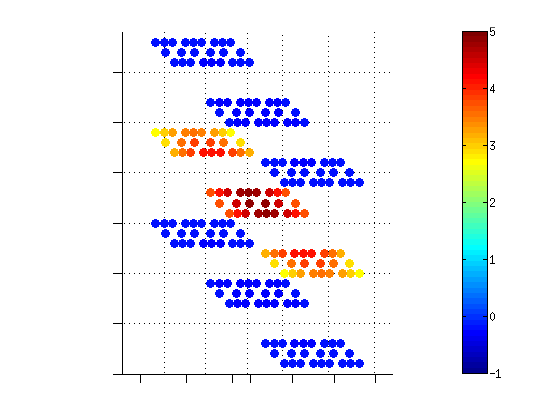
\includegraphics[width=0.75\textwidth]{3D-Surface/figs/attentionmod}
%\makeatletter
%\let\@currsize\normalsize
%\caption[Spread of attention across surfaces]{Spread of attention across surfaces. When attention is directed to the center slanted plane (as in the experiment in Figure 2B-a), attention enhances the activity of all cells along the surface (red), while suppressing the activity of cells belonging to other surfaces (blue).} 
%\label{ModelResults2}
%\end{figure}

\begin{figure}[t]
\centering
\begin{tabular}{c c}
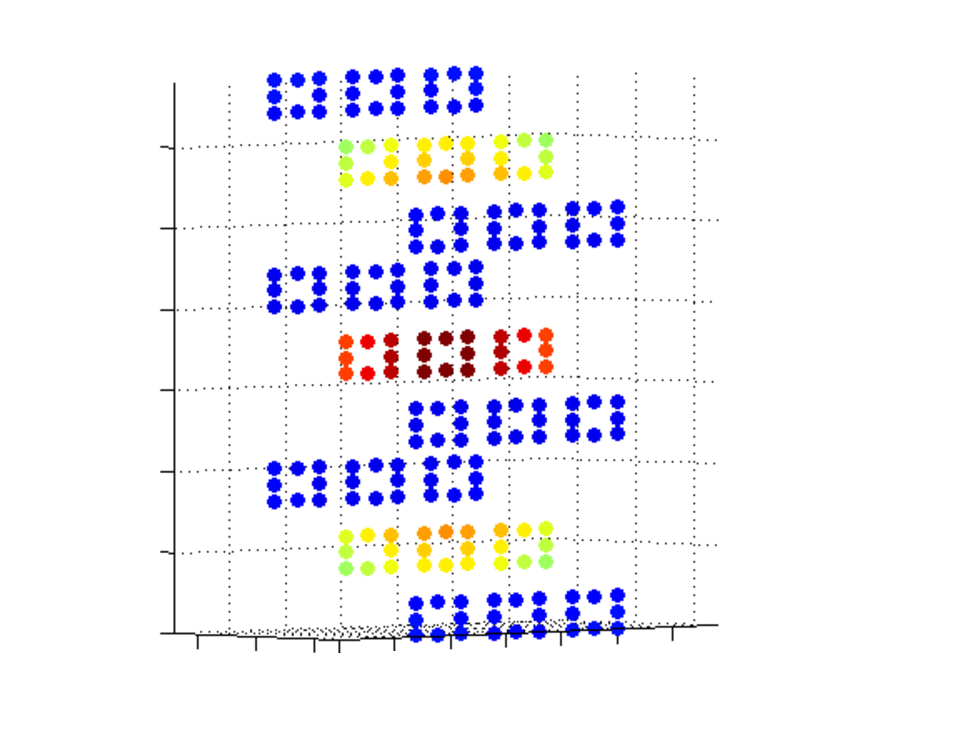
\includegraphics[width=0.5\textwidth]{3D-Surface/figs/2a_nocbar} &
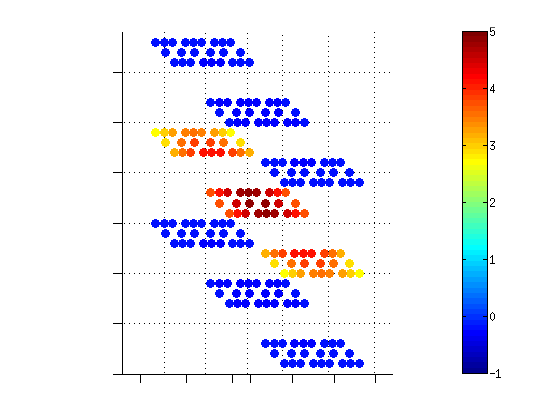
\includegraphics[width=0.5\textwidth]{3D-Surface/figs/attentionmod}\\
(A) & (B)
\end{tabular}
\makeatletter
\let\@currsize\normalsize
\caption[Spread of attention across surfaces]{Spread of attention across surfaces. (A) When attention is directed to the center fronto-parallel plane (as in the experiment in Figure~\ref*{ModelResults}A-a), attention enhances the activity of all cells along the surface (red), while suppressing the activity of cells belonging to other surfaces (blue). (B) Similar results also hold for slanted surfaces in the experiment, Figure~\ref{ModelResults}B-a. The color bar to the right shows attentional modulation over baseline activity, with reddish colors indicating enhancement and bluish colors indicating suppression.}
\label{ModelResults2}
\end{figure}

In our model, we assume that the visual system can selectively direct attention towards a specific surface by providing additional excitatory input to the grouping cell that represents this surface. As shown in Figure~\ref{NetworkStructure}, activity from the grouping cell selectively feeds back to all objects on that surface. In the case of Figure~\ref{ModelResults}A-a, the grouping cell corresponding to the middle fronto-parallel plane receives this attentional input. Activation of the disparity-selective cells in the search plane, shown in Figure~\ref{ModelResults}A-a, bottom row, is thus high. Among the objects in the search plane, the target has a unique color, which results in efficient search and the target being identified immediately. Reaction times are difficult to simulate in detail, therefore the increase in mean activity of disparity-selective cells on the attended plane due to attentional modulation is plotted instead, which is assumed to be inversely proportional to reaction times. The high activation level, bottom row, translates thus into short reaction times, middle row.

In contrast, in Figure~\ref{ModelResults}A-b, the search plane is no longer a well-formed surface but contains objects that are slanted backwards. Directing attention to the middle fronto-parallel plane then has little effect on the disparity-selective cells in the search plane. Search therefore cannot occur entirely within a single plane of coplanar, grouped elements and becomes inefficient, with much higher reaction times (middle row). These long reaction times are reflected in the low activation level of the disparity-selective cells (bottom row). Figure~\ref{ModelResults}A-c shows the analog result for figure elements that are slanted forward rather than backwards, as in A-b. Again, reaction times are long and population activity is low. 

The result is not restricted to fronto-parallel planes, as similar reaction time results were also found for slanted planes in Figure~\ref{ModelResults}B. When subjects are instructed to search in a plane that is coplanar with the orientation of the figure elements (middle plane in B-a), search is fast (B-a, middle row). In contrast,
when the figure elements do not align with the search plane (top row in B-b and B-c), reaction time is increased (middle row). An unexpected result was that activation levels decrease with increasing angle between search plane and stimulus bars for search in slanted planes (difference between Fig~\ref{ModelResults}B-a and B-c). This may explain the observed differences in reaction time data, although~\citet{He_Nakayama95} did not comment on these differences. Again, under the assumption that reaction times are inversely related to reaction times, the model reproduces human behavior (bottom row).

\begin{figure}[t]
\centering
\begin{tabular}{c c}
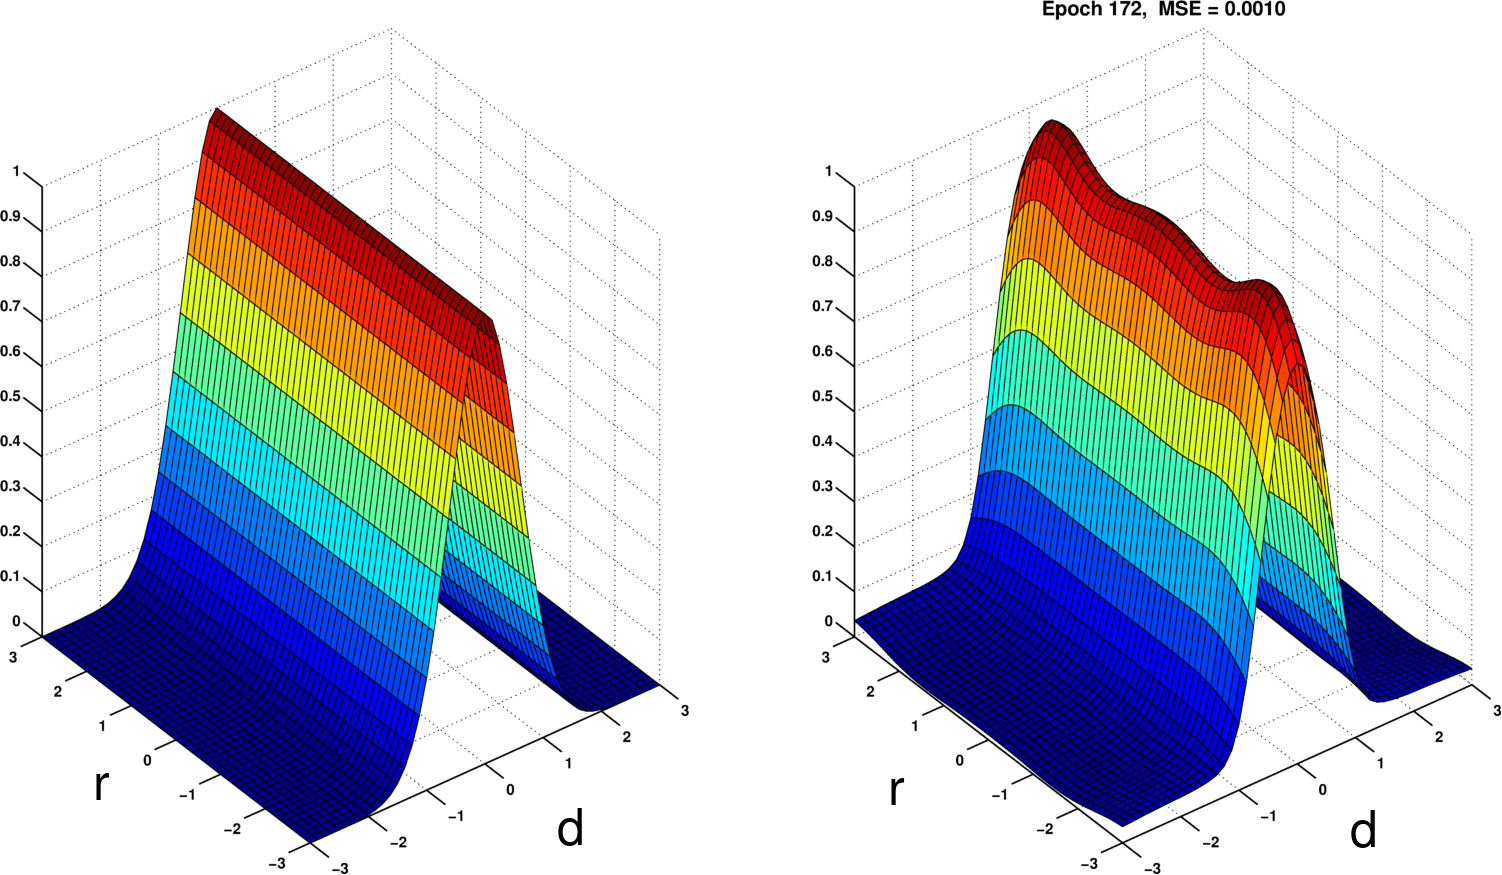
\includegraphics[width=0.45\textwidth]{3D-Surface/figs/frontoparallel} &
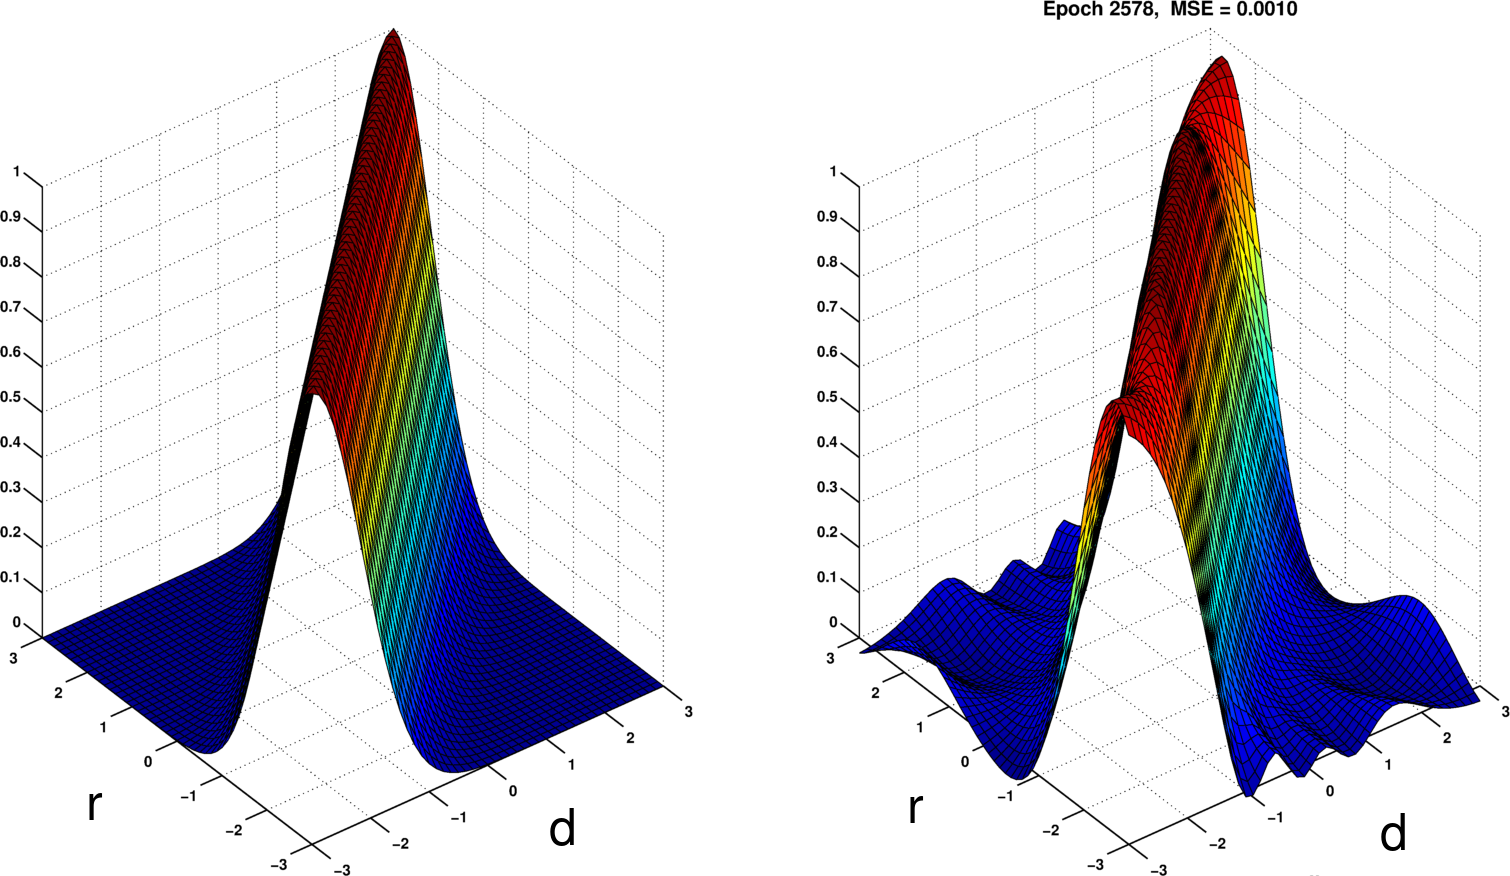
\includegraphics[width=0.45\textwidth]{3D-Surface/figs/slanted}\\
(A) & (B)
\end{tabular}
\makeatletter
\let\@currsize\normalsize
\caption[Comparison of basis function approximation to true surfaces]{Using the same set of basis functions, weights can be learned to approximate different surfaces. (A) Fronto-parallel surface (retinotopic location varies while disparity is constant). The actual surface is shown to the left, and the surface approximation is shown to the right. (B) Similar results also hold for the representation of slanted surfaces (retinotopic location varies with disparity). In each panel, only one retinotopic axis is modeled for ease of visualization.}
\label{Surface_basisfunc}
\end{figure}

\subsection{Spread of attention across surfaces}

In our model, attention can be directed to surfaces, and this is implemented as a top-down input to specific surface grouping neurons. With attention, the neurons encoding the targets within a search array had higher activations when the targets were coplanar with each other and formed a congruent surface, which is consistent with the findings presented in the previous section~\citep{He_Nakayama95}. For both the fronto-parallel surface (Figure~\ref{ModelResults2}A) and the slanted surface (Figure~\ref{ModelResults2}B), top-down attention increased the activity of neurons along the attended surface (shown by the reddish colors), and inhibited the activity of neurons that were not part of the attended surface (shown by the bluish colors). Importantly, the spread of attention was constrained to the surface being attended. In our model, surface grouping neurons are reciprocally connected to disparity-selective neurons coding for targets on a surface. The combination of grouping cells and feature-selective cells represents the presence of ``proto-objects'' in the scene~\citep{Rensink00a}, which results in a structured perceptual organization of the scene in terms of surfaces.

\subsection{Surface representation using basis functions}

In the previous set of results, we represented surfaces using neurons tuned for every possible retinotopic location and disparity. However, this representation is computationally expensive and does not scale well as the size of the input space increases (\ie the number of neurons grows exponentially). Instead, we propose that basis functions may provide a compact and efficient means to represent surfaces using a limited number of neurons. Using our proposed basis function units, which are a function of retinotopic location and disparity (Section~\ref{sec:basis_func}), we were able to learn the weights for two different types of surfaces. 

Figure~\ref{Surface_basisfunc} shows the surface representations approximated by our basis function units. We first determined a set of weights that could approximate the fronto-parallel surface (Figure~\ref{Surface_basisfunc}A). The final approximation had a MSE of 0.001, demonstrating that the units we used form a set of basis functions that could accurately approximate the surface. We then repeated the procedure to determine a set of weights that could approximate the slanted surface (Figure~\ref{Surface_basisfunc}B), which again reached a mean squared error of 0.001. Our results show that both the fronto-parallel and slanted surfaces could be flexibly represented using the same set of basis functions. In our model, these two surface representations coexist, along with an infinite number of other other potential surfaces, which would be represented by different sets of weights. Importantly, any surface can be represented by a single learned linear projection of the basis function units.

\section{Discussion}

As in our previous models, grouping cells serve as ``handles'' for selective attention but now attention is directed not to individual objects but to sets of objects organized in planes. Reaction times were fastest when the search array was a well-formed surface defined by locally coplanar elements. When search array elements were slanted away from this surface, reaction times increased. These results suggest that attention is linked to and spreads across perceived surfaces, which organize the visual scene
(Figure~\ref{ModelResults2}). Our model also makes non-trivial predictions about mean firing rates. Responses of neurons to stimuli in 3D planes should become enhanced, relative to when the stimuli are not part of perceived planes. Furthermore, top-down attention (when cued to a certain plane) provides additional input to G cells and the feedback should enhance responses of neurons in the attended vs. unattended planes.

\subsection{Extension to other surface grouping phenomena}

Grouping implies segregation of some units from others: figure vs. ground, vase vs. face, or, in this case, objects in one plane vs. objects in another plane. In our model, the combination of feedforward grouping with local inhibition allows for local winner-take-all behavior: objects within a plane (or close to it, see below) are grouped together and this group is segregrated from objects further away. If the latter are outside the inhibitory range of the first plane and, of course, arranged themselves in a plane, they will be grouped in a plane of their own. Although we did not explicitly model recurrent local excitation, this may possibly be related to the reverberation needed to explain perceptual persistence.~\citet{McCarley_He01} have found surface priming effects during a similar visual search task, in which the organization of the stimulus array on a previous trial can affect reaction times on the following trial. Related to the idea of local excitation and long-range inhbition, surface grouping cells can excite “close” grouping cells and inhibit “far” grouping cells based on the width of the excitation and inhibition profile. This creates the possibility of depth attraction and repulsion effects, which have been found for isolated dot stimuli as well as random dot stereograms~\citep{Stevenson_etal91}. Extending our model to account for these other phenomena is an area of future research.

\subsection{Generality of basis functions}

Among neurons in striate and extrastriate cortex there are many that respond selectively to stereoscopic disparity~\citep{Poggio_Fischer77,Cumming_DeAngelis01} and they must play a role in the organization of stimuli in 3D space. We propose that the exact same theoretical framework proposed for implementing sensorimotor coordinate transformations in parietal cortex~\citep{Salinas_Abbott95,Pouget_Sejnowski97b} can be used to generate surface grouping cells that represent planes of arbitrary orientations in 3D space. Going from one to the other is a simple affine transformation achieved through combination of neurons with gain field-like receptive fields, and the coefficients of this mapping can be learned by simple, Hebbian-type learning rules. We also note that a surface grouping cell groups all stimuli in the plane it represents, irrespectively of stimulus features (both black and white bars are grouped in planes in Figure~\ref{ModelResults}). It remains to be seen whether surface grouping neurons learned using the basis functions we proposed can also model results from the~\citet{He_Nakayama95} experiments.

Even though surfaces can be represented efficiently with basis functions, one might expect a problem due to the potential inflation of the number of grouping cells to cover all of 3-dimensional space. We have argued that to tile the 2D plane, the number of grouping cells is at least two orders of magnitude smaller than that of B cell~\citep{Craft_etal07}. Even assuming this ratio, the situation seems more difficult in 3D: it appears as if an exceedingly large number of G cells would be required if each plane of any possible orientation (tilt and slant) and any possible depth needs to be explicitly represented by a grouping cell (or a population thereof). This would be a problem for the biological system as well as for our computational model.

Although the number of physical depth planes is obviously infinite, there is no need for them to be explicitly represented at any given time. Indeed, behavioral evidence indicates that only a limited number of depth planes can be perceived in any given situation, up to six with experienced observers being allowed several seconds viewing time, allowing for many eye movements~\citep{Tsirlin_etal08}. The brain must have finer-grained representations of objects in space but those are likely in structures like parietal cortex or hippocampus~\citep{Manns_Eichenbaum09,Deshmukh_Knierim13} and not in visual cortex. We are not aware of any quantitative studies that have measured the number of tilted, or slanted, planes that can be perceived simultaneously, but from our model, we predict that this number is small, too. This is an experimental prediction that should be tested.

\section{Conclusion}

Using a simple model of perceptual organization in 3D,  we are able to reproduce psychophysical results from a visual search task that required allocation of selective attention to surfaces within the scene. The same grouping cells which organize the scene into planes also act as ``handles'' for top-down selective attention, enhancing the activity of coplanar elements belonging to the plane. Competition between grouping cells results in surface enhancement of the plane corresponding to the attended grouping cell, and suppression of other planes within the scene. Our proposed surface representation aids visual processing by providing a critical link between low-level visual features and high-level object representations.

We also show that basis functions, which have traditionally been used to model coordinate transformations between different reference frames, can also provide a flexible and efficient representation of surfaces. Using the same set of basis function units tuned for retinotopic location and disparity, we can potentially represent an infinite number of surfaces using a learned set of weights. This provides a powerful theoretical framework for how the brain may encode a large number of possible surfaces with only a small population of neurons.

%%% Local Variables:
%%% mode: latex
%%% TeX-master: "../root"
%%% End: